\section{Постановка задачи.}
Рассмотри разгон жидкости в плоском канале (Рис. \ref{fig:1}). Разгон происходит за счет действия градиента давления ($\frac{1}{\rho}\frac{\partial{p}}{\partial{x}}$).

\begin{figure}[H]
    \centering
    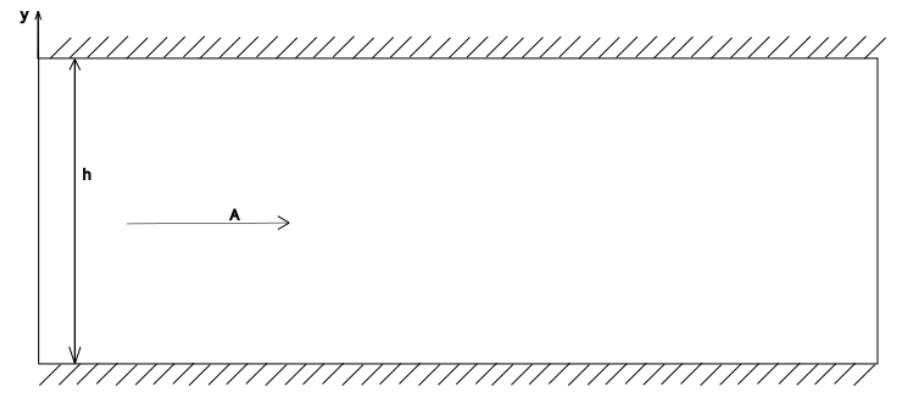
\includegraphics[width=0.5\textwidth]{images/1.png}
    \caption{Схема расчетной области.}
    \label{fig:1}
\end{figure}

Исследуемое течение описывается уравнением (\ref{eq:1}), где $\frac{1}{\rho}\frac{\partial p}{\partial x}=A, [\text{м/с}^2]$ - амплитуда;
$\nu, [\text{м}^2/\text{с}]$ - коэффициент кинематической вязкости; $h, [\text{м}]$ - высота зазора; $u(y,t), \text{м/с}$ - скорость жидкости в точке $(y)$ в момент времени $(t)$; $y, [\text{м}]$ - координата вдоль сечения; $t, \text{с}$ - время.    

\begin{equation}
    \frac{\partial u}{\partial t}-\frac{\partial}{\partial y} \left( \nu \frac{\partial u}{\partial y} \right)-\frac{1}{\rho}\frac{\partial p}{\partial x} = 0
\label{eq:1}
\end{equation}

Начальные условия для задачи - уравнение (\ref{eq:2}). 

Граничные условия для задачи - уравнение (\ref{eq:3}).

\begin{equation}
    u(y,0) = 0
\label{eq:2}
\end{equation}

\begin{equation}
    u(0,t) = 0 ~~~~~~u(h,t) = 0
\label{eq:3}
\end{equation}

В данной задаче нам требуется: рассчитать утановившееся течение; оценить за какой интервал времени оно станет установившимся;
расчитать течение при различных значениях $A$; построить зависимость максимальной скорости при установившемся течении от $A$.

\section{Описание используемых численных методов.}

Для решения поставленной задачи воспользуемся двумя схемами численных методов:
\begin{itemize}
    \item Явная центральная схема.
    \item Явная центральная схема с компенсацией старшего слагаемого ошибки аппроксимации.
\end{itemize}

\subsection{Явная центральная схема.}
Разобьем интервал $[0,h]$ на $N$ узлов с координатами $y_i, i=[1,N]$. Также будет двигаться по временным слоям с шагом по времени $\Delta t$, тогда получим $t^n = n \cdot \Delta t$. 
Будем считать значение на новом слое, основываясь на значении на предыдщуем слое, а также двух соседних точек предыдущего слоя. Граничные условия помогут заполнить значения для крайних узлов интервала. (Рис. \ref{fig:2})
\begin{figure}[H]
    \centering
    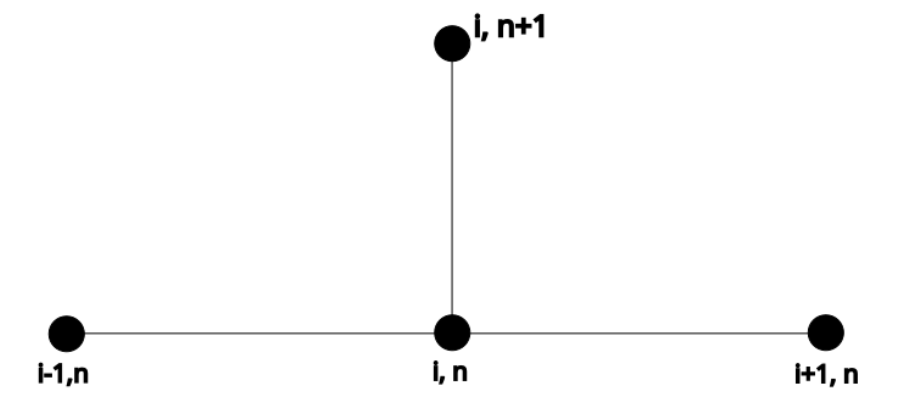
\includegraphics[width=0.5\textwidth]{images/2.png}
    \caption {Шаблон явной центральной схемы.}
    \label{fig:2}
\end{figure}

Аппроксимируем первую производную по времени и вторую по координате, используя ограничение на шаг аппроксимации по времени - $\Delta t \leq \frac{\Delta x^2}{2\nu}$. 
Такое ограничение вводится с целью сохранения устойчивости схемы, как раз таки из-за этого ограничения вычисления при помощи данной схемы являются ресурсоемкими. Это в свою очередь является большим минусом.
Схема аппроксимации представлена в уравнении (\ref{eq:4}).
Также отдельно рассмтарим случай, когда с целью повышения точности аппроксимации выберем такое $\Delta t \leq \frac{\Delta x^2}{6\nu}$.

\begin{equation}
    \frac{u^{n+1}_i-u^n_i}{\Delta t} - \nu \frac{u^n_{i-1}-2u^n_i+u^n_{i+1}}{\Delta y^2} - A =0
    \label{eq:4}
\end{equation}

Теперь аппроксимируем начальные и граничные условия, учитывая, что мы используем N узлов - НУ: $u^1_i = 0, i=[1,N]$; ГУ: $u^n_1 = 0, n - \text{любое} $ $u^n_N = 0, n - \text{любое}$. 

\subsection{Явная центральная схема с компенсацией старшего слагаемого ошибки аппроксимации.}
При использовании явной схемы возникает накапливающаяся ошибка, которая может вредить решению, чтобы этого избежать требуется ее компенсировать. Это нам позволяет разложение функции в ряд Тейлора и отбрасывание величин большего порядка малости, чем в обычной явной схеме. Отсюда у нас появляется еще одно слагаемое. Уравнение данной схемы представлено в уравнении (\ref{eq:5}).
\begin{equation}
    \frac{u^{n+1}_i-u^n_i}{\Delta t} - \nu \frac{u^n_{i-1}-2u^n_i+u^n_{i+1}}{\Delta y^2} + \left[-\frac{\nu^2 \Delta t}{2} + \frac{\nu \Delta y^2}{12} \right] \frac{u^n_{i+2}-4u^n_{i+1}+6u^n_i-4u^n_{i-1}+u^n_{i-2}}{\Delta y^4} = A
\label{eq:5}
\end{equation}

Аппроксимация производных, а также граничных и начальных условий аналогичны явный центральной схеме. Шаблон схемы с учетом старшего слагаемого ошибки аппроксимации представлен на Рис. \ref{fig:3}

\begin{figure}[H]
    \centering
    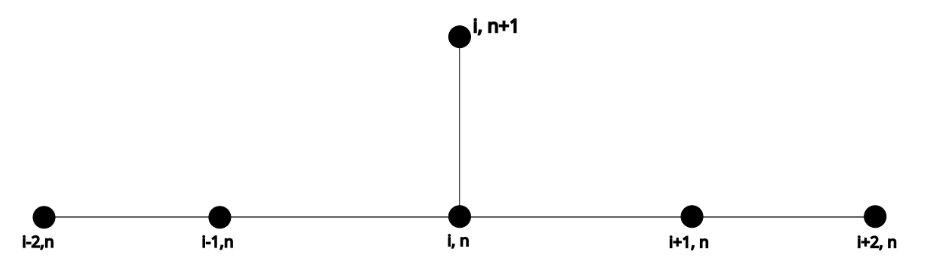
\includegraphics[width=0.5\textwidth]{images/3.png}
    \caption {Шаблон явной центральной схемы с компенсацией.}
    \label{fig:3}
\end{figure}

Но что происходит на границе области, когда мы должны воспользовать для расчетом точками. кторые выходят из нашего диапазона? Введем минимые точки $u^n_0$ и $u^n_{N+1}$. Которые определяются из граничных условий для крайних точек области, а именно: $\frac{\partial^2 u}{\partial y^2}\vert_{y=0,h}=0$. Аппроксимируем данное условие и получим следующее:
\begin{equation}
    \frac{u^n_0-2u^n_1+u^n_2}{\Delta y^2}=0
\label{eq:6}
\end{equation} 

\begin{equation}
    \frac{u^n_{N+1}-2u^n_N+u^n_{N-1}}{\Delta y^2}=0
\label{eq:7}
\end{equation}

Откуда мы найдем значения для наших точек на $n$ слое.


\section{Реализация численного метода.}
Реализуем численный метод, используя язык программирования Fortran. Программа автоматически считывает из текстового файла константы, использующиеся при вычислении скорости на новом временном слое.
Затем она инициализирует начальные условия заданные в программе и начинает итерационно идти вдоль временной координаты, доходя до слоя, в котором значение времени равно времени, заданному предварительно (время, в которое мы хотим получить распределение скорости).
Производится подсчет каждого последующего временного слоя и после достижения заданного времени выводятся значения слоя в документ. Блок схема программы представлена на Рис. \ref{fig:4}.

\begin{figure}[H]
    \centering
    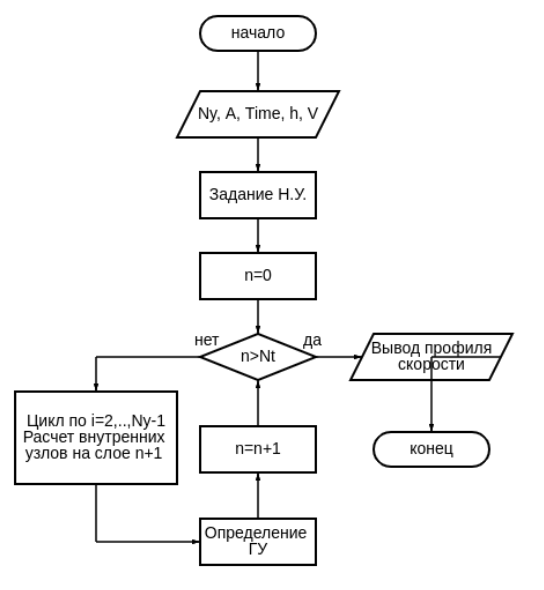
\includegraphics[width=0.5\textwidth]{images/4.png}
    \caption {Блок схема программы реализующей численный метод.}
    \label{fig:4}
\end{figure}

\section{Реализуемый вариант расчетов.}
Будем рассматривать задачу для следующих вводных параметров:
\begin{itemize}
    \item $h=0.01$м - высота зазора
    \item $\nu = 1.e-6 \text{м}^2/\text{с}$  - кинематическая вязкость
    \item $Time = 100$ с - рассматриваемое время течения
    \item $A=0.3 \text{м}/\text{с}^2$ - амплитуда
    \item $Ny = 100$ - количество узлов
\end{itemize}

\section{Результаты расчетов.}
Расчитанное установившееся течение представлено на Рис. \ref{fig:5} (используем визуализатор gnuplot).
Ввиду того, что отличие между схемами является малым, приблизим участок в середине сечения, чтобы визуально наблюдать различия. (Рис. \ref{fig:6})
\begin{figure}[H]
    \centering
    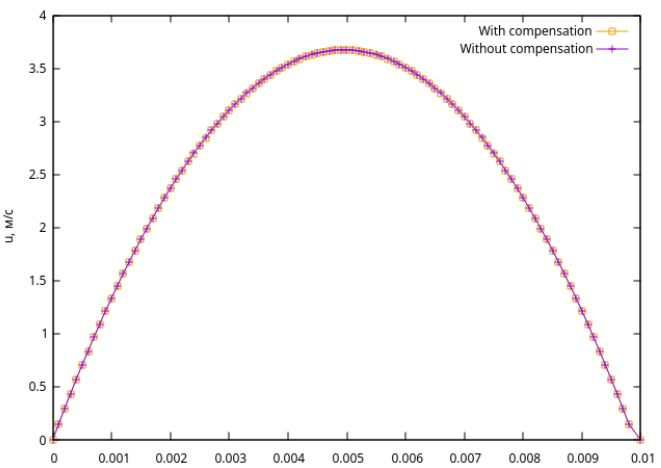
\includegraphics[width=0.5\textwidth]{images/5.png}
    \caption {Профиль скорости установившегося течения.}
    \label{fig:5}
\end{figure}

\begin{figure}[H]
    \centering
    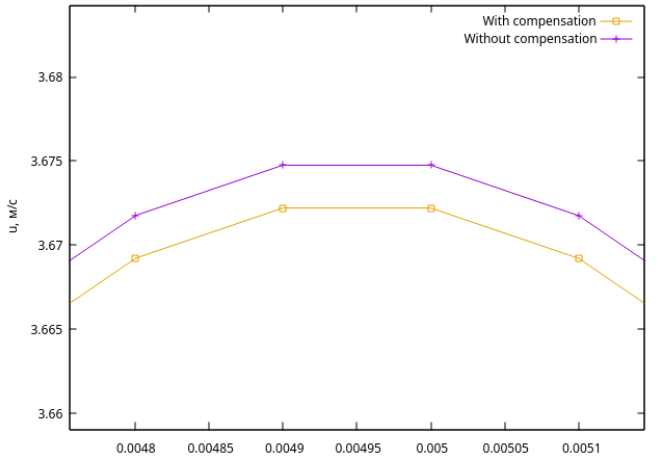
\includegraphics[width=0.5\textwidth]{images/6.png}
    \caption {Различие между двумя схемами.}
    \label{fig:6}
\end{figure}

Из Рис. \ref{fig:6} можем наблюдать, что схемы отличают на значение порядка $10^{-3}$, что говорит о малом их различии.

Время установления течения для явной схемы без компенсации $T_\text{уст}=66.1 \text{с}$, а для схму с учетом компенсации $T_\text{уст}=65.0 \text{с}$. 
Рассмотрим различные значения $A$ и построим для них профили скорости. (Рис. \ref{fig:7}) Как мы можем наблюдать чем больше значение A, тем выше максимум нашей параболы Пуазейля. Действительно, A - ускорение, которое прикладывается к потоку и чем оно больше, тем больше сила, действующая на него, а значит и поток достигает большей скорости, перед тем, как за счет сил сопротивления компенсировать эту движущую силу. 

\begin{figure}[H]
    \centering
    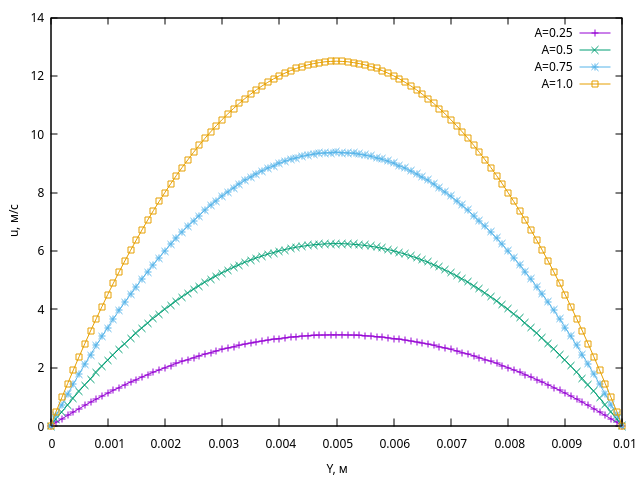
\includegraphics[width=0.5\textwidth]{images/7.png}
    \caption {Графики профиля скорости в зависимости от параметра $A$.}
    \label{fig:7}
\end{figure}

Построим зависимость максимальной скорости от значения параметра $A$. График зависимости представлен на Рис. \ref{fig:8}. Из графика видно, что зависимость максимальной скорости от параметра $A$ является линейной. 
\begin{figure}[H]
    \centering
    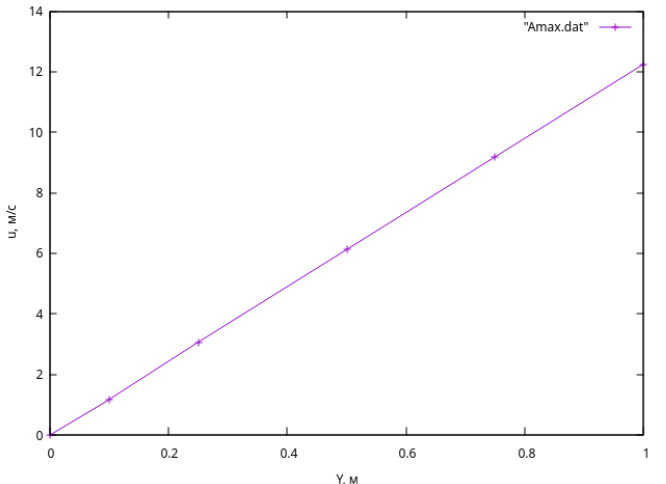
\includegraphics[width=0.5\textwidth]{images/8.png}
    \caption {Графики профиля скорости в зависимости от параметра $A$.}
    \label{fig:8}
\end{figure}

Сопоставим результат полученный с помощью данных схем и аналитическое решение. Аналитическое решение описывается уравнением (\ref{eq:8}).
Визуализация полученных профилей представлена на Рис. \ref{fig:9}.

\begin{equation}
    u=\frac{A}{2\nu} (R^2-r^2), \text{где R=h/2, r=|y-h/2|}
\label{eq:8}
\end{equation}


\begin{figure}[H]
    \centering
    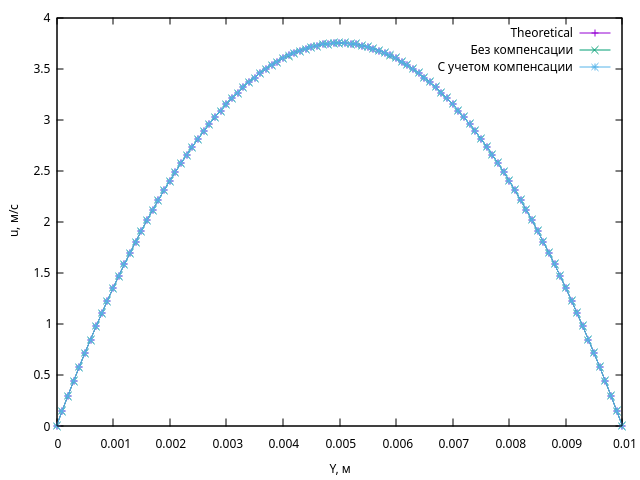
\includegraphics[width=0.5\textwidth]{images/9.png}
    \caption {Сравнение аналитического и численно полученного профилей скорости.}
    \label{fig:9}
\end{figure}

Отличие аналитического решения от численного для обеих схем составляет порядка $\delta = 4\%$ - максимальное отклонение численного решения от аналитического (\ref{eq:9}).

\begin{equation}
    \delta = max\left| \frac{u_i^\text{числ}-u^\text{теор}(y_i)}{u^\text{теор}(y_i)}\right|
\label{eq:9}
\end{equation}

\section{Код программы.}
Код программы представлен в удаленном репозитории на GitHub \\ (https://github.com/MrDionisio/CFD)



\section{Вывод.}
\begin{itemize}
    \item Явная центральная схема без и с компенсацией старшего слагаемого ошибки аппроксимации отличаются друг от друга на 3\%, что говорит нам о том, что данные схемы идентичны и дают одинаково точные результаты.
    \item Полученные профили скорости совпадают с теоритическими расчетами с относительной погрешность максимального отклонения $\delta = 4\%$.
    \item При увеличении параметра амплитуда $A$ максимальная скорость утсановишегося течения растет, причем ее рост является линейным. (Рис. \ref{fig:8})
    \item Полученные профили описывают параболу Пуазейля.
    
\end{itemize}